\documentclass[../main.tex]{subfiles}

\begin{document}

\begin{figure}[h]
    \centering
    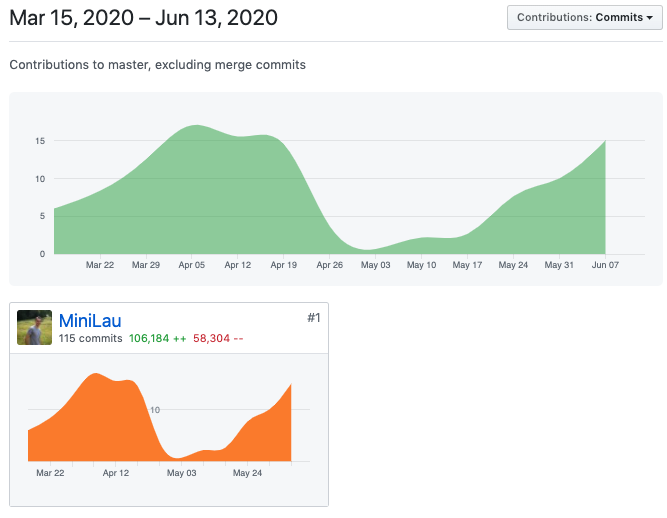
\includegraphics[width=\textwidth]{images/appendix/github_contribution}
    
    \caption{Github code evolution}
    \label{appendix:figure:github_contribution}
\end{figure}

\par \href{https://github.com/MiniLau/Lauxus}{LAUXUS}\footnote{Github repository: \href{https://github.com/MiniLau/Lauxus}{https://github.com/MiniLau/Lauxus}} is written fully in C++ but using only using few C++ functionalities (e.g: we don't use template, etc). In the end, it has over six thousands lines of code with unit testing included. We designed our code to be split into two main folders. One which holds all the source code of the trusted application (code run inside the Enclave) and one for the source code of the untrusted application (code run outside the Enclave). I found that this structure was best suited as at the end, there were way too many files to have them all inside a single folder. Plus, mixing both codes in the same folder was extremely confusing as we no longer understand where the code we write will be running (either in the Enclave or the untrusted application). 
\par By observing Figure \ref{appendix:figure:github_contribution}, we see that the base code of the application required two highly intensive months. Furthermore, I wasn't able to track before March because my git was corrupted and I had to delete it all and solve the issues by hand. On top of that, these two months doesn't take into account the time taken to: understand the required design, understand how to develop with \textit{FUSE} and SGX Enclaves and understanding all the other smaller requirements.
\par However, I like to point that before working on LAUXUS, I worked on some smaller Enclave project to understand how Enclaves worked. I found that SGX development doesn't have at all an easy learning curve even though I have a lot of experience in developing. I realise that because even after a few months working on LAUXUS, there were still things that I didn't understand about Enclaves (mainly on how to write clean code and properly using ECALLS and OCALLS).

\end{document}